\documentclass{beamer}
\bibliographystyle{amsalpha}
\usepackage{cite}
\usepackage[normalem]{ulem}
\setbeamertemplate{footline}[frame number]{}
\setbeamertemplate{navigation symbols}{}

\title{The Heterogeneous Multiscale Method for Plasma Modeling}
\author[Price and Shohet]{Jake Price and Gil Shohet}
\institute[CPSSW]{Computational Physics Student Summer Workshop}
\date{\today}

\begin{document}
\begin{frame}
\titlepage
\end{frame}

\begin{frame}
\frametitle{What is multiscale?}
\begin{columns}[T] 
\begin{column}{.48\textwidth}
\vspace{0.9cm}
``[Multiscale methods] include analytical and numerical techniques that exploit the disparity of scales, as well as multi-physics problems...What we have in mind are problems that involve physical laws at different levels of detail, such as quantum mechanics and continuum models.''\\
\hfill
\\\hfill-Weinan E
\end{column}%

\hfill%

\begin{column}{.48\textwidth}
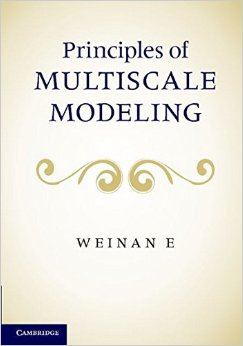
\includegraphics[width=\textwidth]{principles.jpg}
\end{column}%
\end{columns}
\end{frame}

\begin{frame}
\frametitle{What is heterogeneous multiscale method?}
``HMM is a framework for linking models at different scales. It follows a top-down strategy: The basic starting point is an incomplete macroscale model, with the microscale model used as a supplement. It consists of two main components: The macroscale solver and a procedure for estimating the missing numerical data from the microscale model."\\\hfill\\\hfill -Weinan E, et. al.
\end{frame}

\begin{frame}
\frametitle{Our goal}
\begin{itemize}

\item Establish a computational framework for multiscale plasma modeling as a proof of concept
\vspace{1em}
\item Macroscopic model: Kinetic theory using the BGK approximation of the Boltzmann equation (BGK)
\vspace{1em}
\begin{itemize}
\item Relaxation time $\tau$ is an unknown parameter that is typically handled in an ad hoc manner
\end{itemize}
\vspace{1em}
\item Microscopic model: Molecular dynamics (MD)
\vspace{1em}
\begin{itemize}
\item $\tau$ should appear as some sort of average quantity in the MD scale
\end{itemize}



\end{itemize}
\end{frame}




\begin{frame}
\frametitle{Connecting the macroscale to the microscale}
\begin{itemize}
\item We can simulate the molecular dynamics in full detail, but it is much more computationally expensive than the BGK simulation\end{itemize}



\begin{itemize}
\item Idea: Use short MD simulations to approximate relaxation time $\tau$ for use in BGK simulations on a macroscopic timescale
\end{itemize}
\begin{center}
\includegraphics[width=0.3\textwidth]{lightbulb.jpg}\end{center}
\end{frame}



\begin{frame}
\frametitle{Challenges}
\hspace*{3.5em}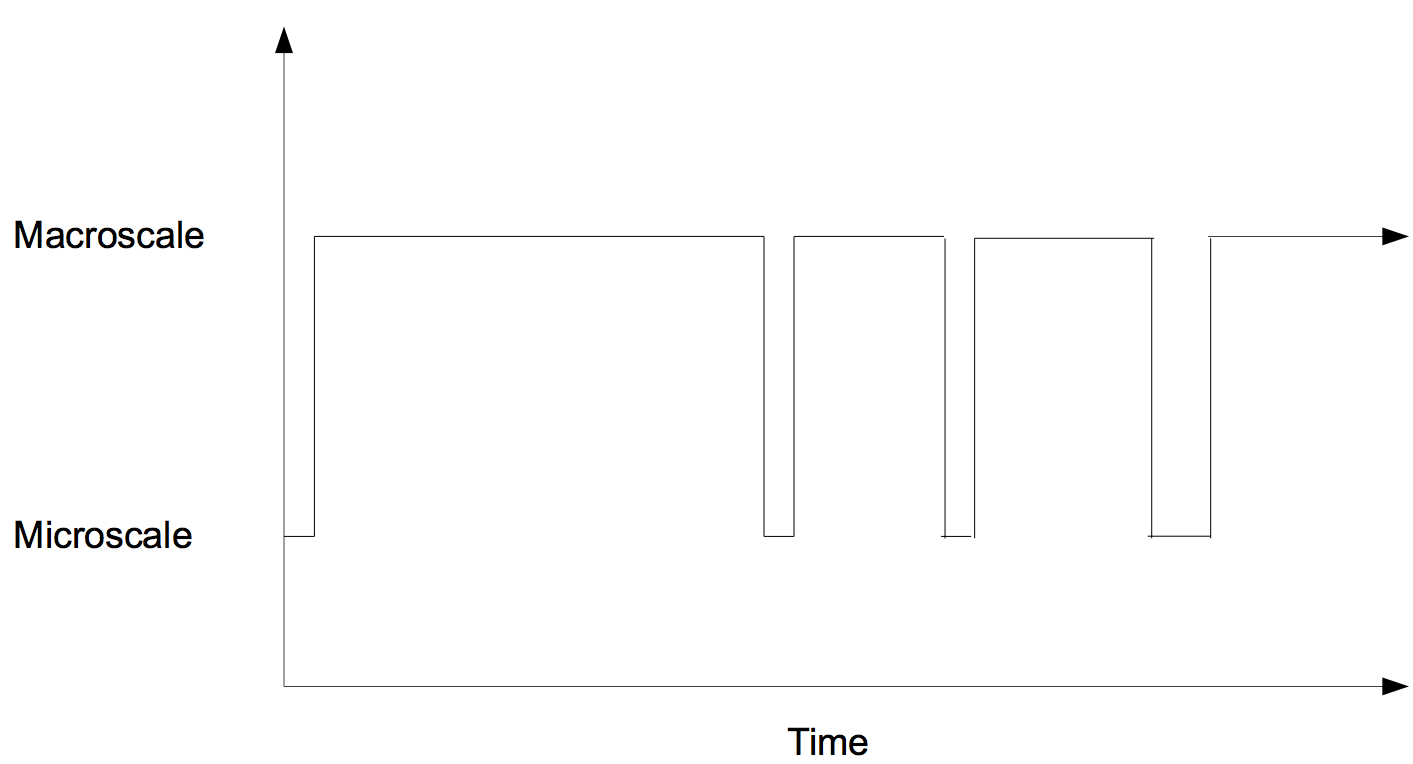
\includegraphics[width=0.65\textwidth]{scheme.png}
\begin{itemize}
\item How to compute $\tau$ from the microscale simulation?
\item How long to run the microscale simulation for reliable $\tau$?
\item How long to run macroscale simulation before returning to update $\tau$?
\item How to downsample the macroscale distribution for a microscale initial condition?
\end{itemize}
\end{frame}



\begin{frame}
\frametitle{Where we are now}
\begin{itemize}
\item At present, we have working code for simulating MD with two spatial and two velocity dimensions, as well as for simulating BGK with one spatial and two velocity dimensions
\vspace{1em}
\begin{itemize}\item Both can take a variety of initial conditions, including $n$ species with different masses and charges (i.e. for a mixing problem)\vspace{1em}
\end{itemize}

\item The code is being tested for bugs, and we will soon begin linking the two
\vspace{1em}
\item Our goal is to choose a regime in which the MD simulation can be computed in full over a long time period, and compare this against a (much faster) multiscale scheme
\end{itemize}
\end{frame}

\begin{frame}
\begin{center}\huge Questions?\end{center}
\end{frame}


\end{document}